
\begin{keynote}
    {Human auditory communication – from visual face areas to sensory thalamus}
    {Katharina von Kriegstein}
    {Friday 11:00 - 12:00 | ORT}
    {Technische Universität Dresden}

    Understanding what is said and recognising the identity of the speaker are two important tasks that the human brain is faced with in auditory communication. For a long time, neuroscientific models of auditory communication have focused mostly on auditory language and voice-sensitive cerebral cortex regions to explain speech and voice identity recognition. However, we now know that the brain uses even more complex processing strategies for recognising auditory communication signals, such as the recruitment of dedicated visual face areas, as well as subcortical sensory thalamus structures. In the first part of my talk, I will present a short overview on our neuroscientific findings how visual face areas help processing auditory communication signals. I will also show studies that translate the neuroscience findings to computational models. In the second part, I will focus on the contribution of subcortical sensory thalamus structures to speech recognition. I will review 7-Tesla neuroimaging findings from typically developed participants as well as developmental dyslexics that suggest a major role of the sensory thalami in speech recognition.

    \vspace*{1cm}

    \begin{figure}[H]
        \raggedleft
        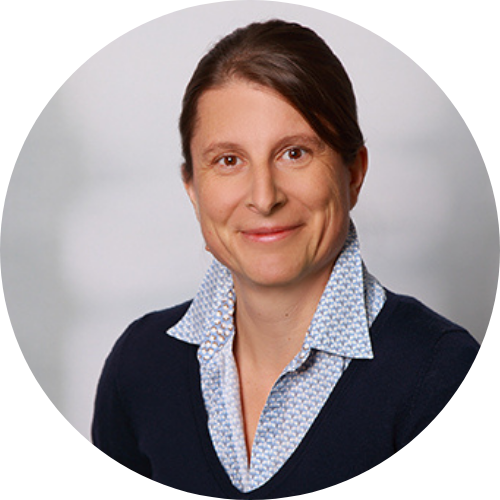
\includegraphics[width=0.24\textwidth]{tex/images/keynote_speaker/kriegstein_cropped.png}
    \end{figure}

\end{keynote}
